\documentclass[tikz,border=10pt,12pt]{standalone}
% Shared preamble for standalone-compiled dc_paper figures.
% Copies just the bits of dc_paper.tex's preamble that figures need.

\usepackage{amsmath,amssymb,amsthm,mathtools,bm}
\usepackage{siunitx}
\sisetup{detect-all,group-separator={,},per-mode=symbol}

\usepackage[T1]{fontenc}
\usepackage{xcolor}
\usepackage{enumitem}
\usepackage{mathpazo}                % Palatino body + matching math
\usepackage[scaled=0.92]{helvet}     % Helvetica sans
\usepackage{courier}                 % monospace
\usepackage{microtype}

% --- IA brand colour palette (must match dc_paper.tex) ---
\definecolor{iadark}{HTML}{1B1815}
\definecolor{iabone}{HTML}{FAFAF7}
\definecolor{iaaccent}{HTML}{A04A1F}
\definecolor{iataupe}{HTML}{F2EDE6}
\definecolor{iarule}{HTML}{3A332D}
\definecolor{iagrey}{HTML}{5A524A}

% --- graphics ---
\usepackage{tikz}
\usepackage{circuitikz}
\usepackage{pgfplots}
\pgfplotsset{compat=1.18}
\usetikzlibrary{arrows.meta,positioning,shapes.geometric,calc,fit,
                decorations.pathreplacing,decorations.markings,
                shadows.blur,backgrounds}

% --- math macros from dc_paper.tex preamble (figures use them) ---
\newcommand{\E}{\mathbb{E}}
\newcommand{\Var}{\operatorname{Var}}
\newcommand{\Cov}{\operatorname{Cov}}
\newcommand{\Cor}{\operatorname{Cor}}
\newcommand{\Prb}{\mathbb{P}}
\newcommand{\R}{\mathbb{R}}
\newcommand{\N}{\mathbb{N}}
\newcommand{\1}{\mathbf{1}}
\newcommand{\VaR}{\operatorname{VaR}}
\newcommand{\TVaR}{\operatorname{TVaR}}
\newcommand{\ES}{\operatorname{ES}}
\newcommand{\dd}{\mathrm{d}}
\newcommand{\given}{\,\vert\,}
\newcommand{\set}[1]{\left\{#1\right\}}
\newcommand{\norm}[1]{\left\Vert #1 \right\Vert}
\DeclareMathOperator*{\argmin}{arg\,min}
\DeclareMathOperator*{\argmax}{arg\,max}

% \textwidth has no meaning in standalone class; give it a value matching
% the paper's A4 + 1-inch margins so any leftover \resizebox{\textwidth}
% gracefully sizes the figure to that nominal width.
\setlength{\textwidth}{15.92cm}

\begin{document}
\pagecolor{iabone}
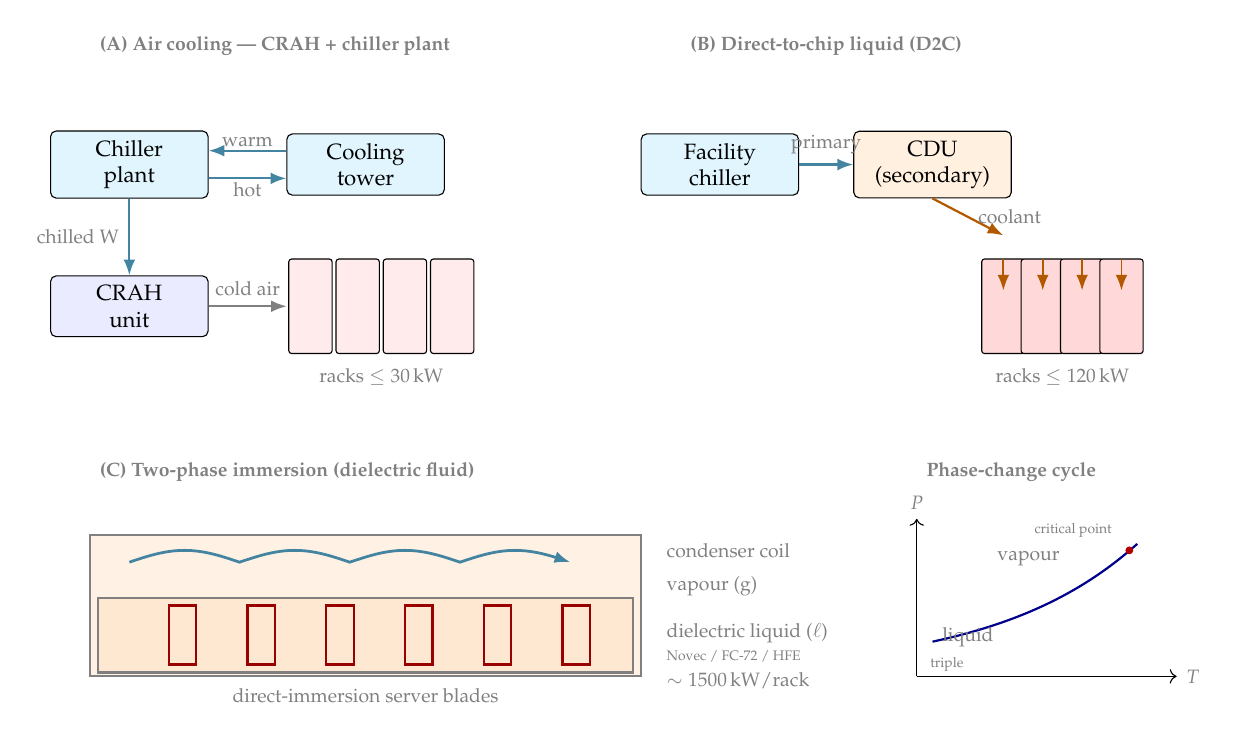
\begin{tikzpicture}[
   every node/.style={font=\footnotesize},
   blk/.style={draw,rounded corners=2pt,minimum width=2.0cm,minimum height=0.65cm,
               align=center,fill=blue!4},
   rack/.style={draw,rounded corners=1pt,minimum width=0.55cm,minimum height=1.2cm,
                fill=red!8,align=center,font=\tiny},
   pipe/.style={thick,blue!55!black,-{Latex[length=2mm]}},
   wpipe/.style={thick,cyan!60!black,-{Latex[length=2mm]}},
   opipe/.style={thick,orange!70!black,-{Latex[length=2mm]}},
   label/.style={font=\scriptsize,gray}
]

% =========== Panel A: Air cooling ============
\node[label,anchor=west,font=\scriptsize\bfseries] at (0,5.0)
   {(A) Air cooling --- CRAH + chiller plant};

\node[blk,fill=cyan!12] (CH) at (0.5,3.5) {Chiller\\plant};
\node[blk,fill=cyan!12] (CT) at (3.5,3.5) {Cooling\\tower};
\node[blk,fill=blue!8]  (CRAH) at (0.5,1.7) {CRAH\\unit};

% Two return/supply pipes separated by 10pt so the arrows don't merge
% and the labels sit cleanly on the outside of each pipe.
\draw[wpipe,transform canvas={yshift= 5pt}] (CT) -- (CH)
   node[midway,above,label,inner sep=1pt] {warm};
\draw[wpipe,transform canvas={yshift=-5pt}] (CH) -- (CT)
   node[midway,below,label,inner sep=1pt] {hot};
\draw[wpipe] (CH) -- (CRAH) node[midway,left,label] {chilled W};

% Server racks (air-cooled)
\foreach \x in {2.8,3.4,4.0,4.6} {
  \node[rack] at (\x,1.7) {};
}
\node[label] at (3.7,0.8) {racks $\leq\SI{30}{\kilo\watt}$};
\draw[pipe,gray] (CRAH.east) -- (2.5,1.7) node[midway,above,label] {cold air};

% =========== Panel B: Direct-to-chip liquid ============
\node[label,anchor=west,font=\scriptsize\bfseries] at (7.5,5.0)
   {(B) Direct-to-chip liquid (D2C)};

\node[blk,fill=cyan!12] (CH2) at (8.0,3.5) {Facility\\chiller};
\node[blk,fill=orange!12](CDU) at (10.7,3.5) {CDU\\(secondary)};
\draw[wpipe] (CH2) -- (CDU) node[midway,above,label] {primary};

% Manifold + cold plates
\foreach \x in {11.6,12.1,12.6,13.1} {
  \node[rack,fill=red!15] at (\x,1.7) {};
  \draw[opipe,line width=0.7pt] (\x,2.3) -- (\x,1.9);
}
\draw[opipe] (CDU.south) -- (11.6,2.6) node[midway,right,label] {coolant};
\node[label] at (12.35,0.8) {racks $\leq\SI{120}{\kilo\watt}$};

% =========== Panel C: Immersion (full width, lower row) ============
\node[label,anchor=west,font=\scriptsize\bfseries] at (0,-0.4)
   {(C) Two-phase immersion (dielectric fluid)};

% Tank, wider
\draw[thick,gray,fill=orange!10] (0,-3.0) rectangle (7,-1.2);
% liquid (lower part)
\draw[thick,gray,fill=orange!18] (0.1,-2.95) rectangle (6.9,-2.0);

% Submerged blades (drawn first so labels can sit beside them)
\foreach \x in {1.0,2.0,3.0,4.0,5.0,6.0} {
  \draw[red!60!black,thick] (\x,-2.85) rectangle (\x+0.35,-2.1);
}

% Condenser coil at top - placed in the vapour space
\draw[wpipe,line width=1.0pt]
  (0.5,-1.55) sin (1.2,-1.4) cos (1.9,-1.55)
              sin (2.6,-1.4) cos (3.3,-1.55)
              sin (4.0,-1.4) cos (4.7,-1.55)
              sin (5.4,-1.4) cos (6.1,-1.55);

% Labels - placed OUTSIDE the busy tank, to the right
\node[label,anchor=west] at (7.2,-1.4) {condenser coil};
\node[label,anchor=west] at (7.2,-1.85) {vapour (g)};
\node[label,anchor=west] at (7.2,-2.45) {dielectric liquid ($\ell$)};
\node[label,anchor=west,font=\tiny] at (7.2,-2.75) {Novec / FC-72 / HFE};
\node[label] at (3.5,-3.25) {direct-immersion server blades};
\node[label,anchor=west] at (7.2,-3.05) {$\sim\SI{1500}{\kilo\watt\per rack}$};

% Phase change diagram (right side)
\node[label,anchor=west,font=\scriptsize\bfseries] at (10.5,-0.4)
   {Phase-change cycle};
\draw[->] (10.5,-3.0) -- (13.8,-3.0) node[right,label] {$T$};
\draw[->] (10.5,-3.0) -- (10.5,-1.0)  node[above,label] {$P$};
\draw[blue!55!black,thick] plot[domain=0.2:2.8,smooth,samples=40]
  ({10.5+\x}, {-2.95+0.35*exp(0.55*\x)});
\node[label,anchor=west] at (10.7,-2.5) {liquid};
\node[label,anchor=west] at (11.4,-1.5) {vapour};
\filldraw[red!70!black] (13.2,-1.4) circle (1.2pt);
\node[label,anchor=east,font=\tiny] at (13.1,-1.15) {critical point};
\node[label,anchor=west,font=\tiny] at (10.55,-2.85) {triple};

\end{tikzpicture}
\end{document}
